
\chapter{New approaches to unsupervised learning}
\label{chap:asmclustering}

This chapter begins with a short overview of various agent-based clustering approaches in Section \ref{sec:agentbased}. The rest of the chapter is entirely original and presents our contribution to agent-based clustering, particularly in two main directions: ASM-based batch clustering and incremental clustering. We are focusing on developing clustering algorithms that allow the discovery and analysis of hybrid data.

The unsupervised learning approaches presented in this chapter are original works published in \cite{Gaceanu10AnAdaptive,  Gaceanu11AContext, Gaceanu11AFuzzy, Gaceanu11ABio, Gaceanu11AnIncremental}. 

The chapter is structured as follows. In Section \ref{sec:agentbased} a short overview of various agent-based clustering approaches is presented. 
We approach the idea of agent-based cluster analysis in Section \ref{sec:asmbasedclustering}. Each data item is represented by an agent placed in a two dimensional grid. The agents will group themselves into clusters by performing simple moves using some local environment information, the parameters being selected and updated adaptively. This behaviour based on ASM (Ant Sleeping Model) where an agent may be either in an active state or in a sleeping state. In order to avoid the agents being trapped in local minima, they are also able to directly communicate with each other. Furthermore, the agent moves are expressed by fuzzy IF-THEN rules and hence hybridization with a classical clustering algorithm is needless. The proposed fuzzy ASM-based clustering  algorithm is presented in Section \ref{sec:fuzzyasmclustering}. 
In this model data items to be clustered are represented by agents that are able to react according to the changes in the environment, namely the number of neighbouring agents. However a change in the data item itself is not handled at runtime. An extension to a context-aware system would be beneficial in many practical situations. 
In general, context-aware systems could greatly change the way we interact with the world --- they could anticipate our needs and advice us when taking some decisions. In a changing environment context-awareness is undoubtedly beneficial.  Such systems could make much more relevant recommendations and support decision making. An extension to a context-aware approach is presented in Section \ref{sec:contextaware}. Case studies for both approaches including experiments on standard datasets \cite{website:iris, website:wine} are presented in Section \ref{sec:caseasm}.
The idea behind incremental clustering is that it is possible to consider one instance at a time and assign it to existing clusters without significantly affecting the already existing structures. Section \ref{chap:incrementalclustering} presents an incremental clustering approach based on ASM. In incremental clustering only the cluster representations need to be kept in memory so not the entire dataset and thus the space requirements for such an algorithm are very small. Whenever a new instance is considered an incremental clustering algorithm would basically try to assign it to one of the already exiting clusters. Such a process is not very complex and therefore the time requirements for an incremental clustering algorithm are also small. The fuzziness of the approach allows the discovery of hybrid data. Experimental evaluation on standard datasets \cite{website:iris, website:wine} are presented in Section \ref{sec:experiments}. Section \ref{sec:clustconclusionsfw} outlines the conclusions of the chapter and indicates some research directions that will be followed.

The original contributions of this chapter are:

\begin{itemize}

\item A fuzzy ASM-based clustering algorithm (Section \ref{sec:fuzzyasmclustering}) \cite{Gaceanu10AnAdaptive, Gaceanu11ABio}.

\item A context-aware fuzzy clustering algorithm (Section \ref{sec:contextaware}) \cite{Gaceanu11AContext, Gaceanu11AFuzzy}.

\item An incremental fuzzy clustering algorithm (Section \ref{chap:incrementalclustering}) \cite{Gaceanu11AnIncremental}.

\item Experimental evaluation of the algorithms on standard datasets (Section \ref{sec:caseasm} and Section \ref{sec:experiments}) \cite{Gaceanu10AnAdaptive, Gaceanu11ABio, Gaceanu11AContext, Gaceanu11AFuzzy, Gaceanu11AnIncremental}.

\item The discovery and analysis of hybrid data (Section \ref{sec:caseasm} and Section \ref{sec:experiments}) \cite{Gaceanu11AContext, Gaceanu11AFuzzy, Gaceanu11AnIncremental}.

\item The applicability of the fuzzy ASM-based methods in clustering web search results (Section \ref{sec:caseasm}) \cite{Gaceanu10AnAdaptive, Gaceanu11ABio}.

\end{itemize}

\section{Agent-based unsupervised learning}
\label{sec:agentbased}
Several clustering algorithms exist each with its own strengths and weaknesses. Some algorithms need an initial estimation of the number of clusters (k-means, fuzzy c-means) while others could often be too slow (agglomerative hierarchical clustering algorithms). Ant-based clustering algorithms often require hybridization with a classical clustering algorithm such as k-means \cite{Schockaert04Fuzzy}. 

In \cite{Chen04AnAdaptive} the authors present an ant-based clustering algorithm. It is based on the ASM (Ants Sleeping Model) approach. 
In the ASM model an ant may be in any one of the following two possible states: active and sleeping.
When the ant's fitness is low, the probability of switching to active state is higher. If this happens the ant will leave its position and it will start to search for a more comfortable position for sleeping, i.e., a position where its fitness is high enough. When a position which increases the ant's fitness has been located it has a higher probability to switch to sleeping state and stay at that position until the environment becomes less hospitable again. 

Based on ASM, the authors present an Adaptive Artificial Ants Clustering Algorithm (A$^{4}$C) \cite{Chen04AnAdaptive} in which every ant is a simple agent that corresponds to an individual data item. ''The whole ant group dynamically self-organizes into distinctive, independent subgroups within which highly similar ants are closely connected. The result of data objects clustering is therefore achieved.'' \cite{Chen04AnAdaptive}. However, by using local information only the risk of getting trapped into local optimum solutions exists.

Another approach to data clustering with ants is the one from the BM \cite{Deneubourg91TheDynamic} and LF \cite{Lumer94Diversity} models which use the ants' behaviour of piling corpses. In this case ants pick up the corpses and put them in piles preferring larger piles. Items can be moved from one pile to another. This model has a  rather high computational time cost because of the idle moves required until an item is found. 

In \cite{Chira07Stigmergic} a Stigmergic Agent System (SAS) combining the strengths of Ant Colony Systems and Multi-Agent Systems concepts is proposed. The agents from the SAS are using both direct and indirect communication. By using direct communication the risk of getting trapped in local optima is lower. However, as showed in \cite{Schockaert04Fuzzy}, most ant-based algorithms can be used only in a first phase of the clustering process because of the high number of clusters that are usually produced. In a second phase a k-means-like algorithm is often used. 

In \cite{Schockaert04Fuzzy}, an algorithm in which the behaviour of the artificial ants is governed by fuzzy IF-THEN rules is presented. 
As in any typical ant-based clustering algorithm, the advantage is that an initial data partitioning is not required and also the number of clusters does not need to be known a prori.
The ants are capable to make their own decisions about picking up items and then the two phases of the classical ant-based clustering algorithm are merged into one, which makes k-means superfluous \cite{Schockaert04Fuzzy}.

In \cite{Gaceanu11AContext}, the clustering problem is approached by the idea of context-aware ASM agents. The agents are able to detect changes in the environment and adjust their moves accordingly. The advantage of this approach is that it enables the  ants to communicate directly like in \cite{Chira07Stigmergic} therefore breaking the neighbourhood boundaries and thus decreasing the chance of ants to get trapped in local minima. The fuzzy IF-THEN rules governing the agents' movements are also allowing the agents to go beyond the neighbourhood limits; for example in the case of two very different ($VD$) agents it makes no point to keep them in a reachability distance; and it makes sense that two very different ($VD$) agents should move further away from each other than two different ($D$) agents do. Thus the system behaves more naturally. The agents are able to adapt their movements if changes in the environment would occur and this is an important feature in real-time systems, wireless sensor networks or data streams.

The skeleton of our approach \cite{Gaceanu10AnAdaptive} is based on the ASM-like algorithm from \cite{Chen04AnAdaptive} embellished with features from \cite{Chira07Stigmergic} and \cite{Schockaert04Fuzzy}. 	
In ASM (Ants Sleeping Model), an ant may be either in active state or in sleeping state. When the artificial ant's fitness is low, it has a higher probability to wake up and stay in active state. It will thus leave its original position to search for a more secure and comfortable position to sleep. When an ant locates a comfortable and secure position, it has a higher probability to sleep unless the surrounding environment becomes less hospitable and activates it again. Ants use only local information in order to switch between states and in time the whole group dynamically self organizes into formations within which similar ants are close to each other and therefore clustering is achieved.   
The definitions \ref{def:grid} -- \ref{def:pa} from bellow are taken from \cite{Chen04AnAdaptive}.

\begin{definition}
\label{def:grid}
The grid in ASM is 
 a two-dimensional array
\begin{align} G(x,y)\epsilon Z ^{+} \bigcup \{0\},     \end{align}  
  of all positions  \begin{align}(x,y) \epsilon [0..2\lceil\sqrt{n}\rceil-1]^{2},\end{align} such that:
\begin{align} 
G(x, y) = 
\left\{
\begin{array}{ll}
		i  & \mbox{if there is an agent labelled $i$ at position $(x, y)$ } \\
		0 & \mbox{otherwise }
	\end{array}
\right.
\end{align}
 
where  $n$ is the number of agents.



\end{definition}


\begin{remark}
The grid size depends on the number of agents and thus we avoid both grid overcrowding and allocating a grid which consumes too many resources.
\end{remark}

\begin{remark}
The ASM uses a grid topologically equivalent to a sphere grid and hence all cells are equal to each other with respect to the number of neighbours. So the cells from the margins have the same number of neighbours as the cells from the interior of the grid, i.e., one can jump from one of the northmost positions to one of the southmost positions with one step. 
\end{remark}


\begin{definition}
In ASM, each agent represents one data item.
Let an agent represent a data item by using  \begin{math}   agent _{i}   \end{math} to represent the \begin{math}   i^{th}     \end{math} agent, and $n$ be the number of agents. The position of an agent is represented by  \begin{math} (x_i,y_i) \end{math}, namely \begin{math} G(agent_i)=G(x_i,y_i)=i   \end{math}
\end{definition}

\begin{definition} 
The  neighbourhood of an agent is
\begin{align}  
N(agent_i)=N(x_i,y_i)=\{(x,y) mod (2\lceil \sqrt{n} \rceil ) | \mid x-x_i \mid \leq s_x ,   \mid y-y_i \mid \leq s_y \}   
\end{align}
\end{definition}

\begin{definition}
The set of empty positions in the neighbourhood is
\begin{align}  
L(agent_i)=L(x_i,y_i)=\{(x,y) | (x,y) \epsilon N(agent_i), G(x,y)=0 \}    
\end{align}
\begin{math}  s_x  \end{math} and \begin{math}  s_y  \end{math} are the vision limits in the horizontal and vertical direction respectively.
\end{definition}

\begin{definition}
The fitness of an agent is
\begin{align}  
f(agent_i)=\frac{1}{(2s_x + 1) (2s_y + 1)} \sum_{agent_j \epsilon N(agent_i)} \frac{\alpha^2}{\alpha^2+d(agent_i,agent_j)^2},
\end{align}  
\begin{align}
\alpha=\frac{1}{n(n-1)} \sum_{i=1}^{n} \sum_{j=1}^{n} d(agent_i,agent_j),
\end{align}  
where:\\
\begin{itemize}
\item $f(agent_i)$ represents the current fitness of agent $i$.
\item $\alpha$ is  the average distance between the agents. 
\end{itemize}
\end{definition}

\begin{remark}
The distance between two agents, $d(agent_i,agent_j)$, is the Euclidean distance between the two agents from the grid.
\end{remark}

\begin{definition}
\label{def:pa}
The activation probability is
\begin{align} 
p_a(agent_i)=cos^\lambda (\frac{\pi}{2}f(agent_i)),
\end{align}
where \begin{math}  \lambda \epsilon R^+  \end{math} is a parameter, and can be called agents' activation pressure.
\end{definition}

\begin{remark}
Function \begin{math} p_a(agent_i)  \end{math} represents the probability of the activation of the agent by the surroundings. If the fitness is low then the probability of activation is high so the agent is probably going to wake up, move and search for a better place to sleep. Conversely if the fitness is high then the probability is low so most probably the agent will stay and sleep.
\end{remark}

The algorithm from \cite{Chen04AnAdaptive} starts by randomly placing the agents on the grid in active state. The agents start to perform simple moves on the grid. Whenever it arrives in a new location the agents updates its fitness and activation probability (defined above). If the activation probability is low then the chances that the agent will stop wandering are higher. If this is the case then the agent will switch to sleeping state and unless the environment becomes less hospitable it will continue to stay in sleeping state at that position. The agents's fitness is related to the number of similar individuals in its neighbourhood. With increasing number of iterations, such movements gradually increase this leading to a clustering in data.


\section{ASM-based clustering}
\label{sec:asmbasedclustering}

In ASM (Ants Sleeping Model), an agent located on a two-dimensional grid may be in any of the following states: active or sleeping. When the agent's fitness is low, it has an increased probability to become  active and start searching for a more comfortable position, where its fitness is increased. When such a position in located, the agent has an  increased probability to move in a sleeping sate until the local environment becomes less hospitable and activates it again.
At the beginning of every considered ASM-based clustering approach the agents are randomly placed on the grid in active state. Whenever an agent move to a new position, it will update its fitness $f_{disim}$ and probability $p_a$ and based on this information it can decide whether it should continue moving or not. While the $p_{a}$ is high the agent is likely to stay active and continue to explore the grid. If the current $p_{a}$ becomes small, the agent has a lower probability to keep exploring the grid so it may stop at the current position and switch to sleeping state. With increasing number of iterations, such movements gradually increase, eventually, making similar agents gathered within a small area and different types of agents located in separated areas. Thus, the corresponding data items are clustered. 

In our ASM approaches we use Definition \ref{def:fitour} for the fitness of an agent.

\begin{comment}

\begin{definition}
The dissimilarity-based fitness of an agent is 
\begin{align} 
f_{disim}(agent_i)=\frac{1}{(2s_x + 1) (2s_y + 1)} \sum_{agent_j \epsilon N(agent_i)} \frac{\alpha^2}{\alpha^2+ disim(agent_i,agent_j) de(agent_i,agent_j)},
\end{align}
\begin{align}
\alpha=\frac{1}{n(n-1)} \sum_{i=1}^{n} \sum_{j=1}^{n} de(agent_i,agent_j),
\end{align}  
where:
\begin{itemize}
\item $de(agent_i,agent_j)$ ---
 represents the euclidean distance between the agents on the grid
\item  \begin{math} 
disim(agent_i,agent_j)
 \end{math}
---  denotes the dissimilarity between the two agents. 

\end{itemize}
\end{definition}

\end{comment}

\begin{definition}
\label{def:fitour}
The dissimilarity-based fitness of an agent is
\begin{align} 
f(agent_i)=\frac{1}{v} \sum_{a_j \epsilon N(a_i)} \frac{\alpha^2}{\alpha^2+ disim(a_i,a_j)de(a_i,a_j)},\\
 \end{align}
\begin{align}
v=\frac{1}{(2s_x + 1) (2s_y + 1)}
\end{align}
\begin{align}
\label{rel:alpha1}
\alpha=\frac{1}{n(n-1)} \sum_{i=1}^{n} \sum_{j=1}^{n} de(a_i,a_j),
\end{align}  
 where:
 \begin{itemize}
\item   $a_i$ and $a_j$ respectively denote $agent_i$ and $agent_j$,
\item $de(a_i,a_j) $  represents the Euclidean distance between the agents on the grid, 
\item $disim(a_i,a_j)$  denotes the dissimilarity between the two agents. 
\end{itemize}
\end{definition}

The activation probability $p_{a}$ is the same as the one from Definition \ref{def:pa}.


\subsection{Fuzzy ASM-based clustering}
\label{sec:fuzzyasmclustering}

The agents decide upon the way they move on the grid based on their similarity with the neighbours, using fuzzy IF-THEN rules. Thus two agents can be similar (S), different (D), very different (VD). If two agents are similar they would get closer to each other. If they are different or very different they will get away from each other. The number of steps they do each time they move depend on the similarity level. So if the agents are $VD$ they would jump many steps away from each other; if they are $D$ they would jump less steps away from each other. In the end the ants which are $S$ will be in the same cluster. The parameter $\alpha$ is the average distance  between agents and this changes at each step further influencing the fitness function. The parameter $\lambda$ influences the agents' activation pressure and it may decrease over time. The parameter $t$ is used for the  termination condition which could be something like \begin{math} t < t_{max}  \end{math}. The parameters $s_x, s_y$, the agent's vision limits, may also be updated in some situations.  

\begin{algorithm}
\caption{Fuzzy ASM Clustering}
\label{alg:fuzzyasmclustering}
\begin{algorithmic}[1]
\STATE initialize parameters  $\alpha, \lambda, t, s_x, s_y$
\FORALL {agent}
	\STATE @ place agent at randomly selected site on the grid
\ENDFOR
\WHILE {not termination}
	\FORALL {agent}
		\STATE @ compute agent’s fitness and activate probability $p_a$ according
						to the definitions from above
		\STATE $r \leftarrow random (0,1)$
		\IF {$r < p_a$} 
			\STATE @ activate agent and move to a site in the neighbourhood based on the similarity with the neighbours using fuzzy IF-THEN rules
		\ELSE
			\STATE @ stay at current site and sleep
		\ENDIF 

	\ENDFOR
	\STATE @ adaptively update parameters $\alpha, \lambda, t, s_x, s_y  $
\ENDWHILE
\end{algorithmic}
\end{algorithm}
\begin{comment}
\begin{algorithm}
{\small \vspace{2 mm} Clustering}
{\small \hspace{4 mm} initialize parameters  $\alpha, \lambda, t, s_x, s_y$}
{\small \hspace{4 mm} for each agent do}
{\small \hspace{8 mm} 	place agent at randomly selected site on the grid}
{\small \hspace{4 mm} endFor}
{\small \hspace{4 mm} while (not termination)}
{\small \hspace{8 mm}	for each agent do}
{\small \hspace{12 mm}		compute agent’s fitness and activate probability $p_a$ according
						to the definitions from above}

{\small \hspace{12 mm}		r $\leftarrow$ random (0,1)}

{\small \hspace{12 mm}		if ($r < p_a$) then} 

{\small \hspace{16 mm} 			activate agent and move to a site in the 
                                                                         neighbourhood based on the similarity with} 

{\small \hspace{18 mm}				the neighbours using fuzzy IF-THEN rules}

{\small \hspace{12 mm}		else} 

{\small \hspace{16 mm} 			stay at current site and sleep}

{\small \hspace{12 mm}		endif}

{\small \hspace{8 mm}	endFor}

{\small \hspace{8 mm} 	adaptively update parameteres $\alpha, \lambda, t, s_x, s_y  $}

{\small \hspace{4 mm} endWhile}

endAlgorithm

\end{algorithm}
\end{comment}

In the following, the fuzzy sets $S$, $D$, $VD$ are defined:
\begin{align}
S, D, VD: X \rightarrow [0,1]
\end{align}
\begin{align}
S(x) = \left\{
     \begin{array}{lr}
       1 & , x \in [0, SD1]\\
       (SD1-x)+1 & , x \in [SD1, SD2]\\
       0 & , otherwise
     \end{array}
   \right.
\end{align}

\begin{align}
D(x) = \left\{
     \begin{array}{lr}
       (x-SD2)+1 & , x \in [SD1, SD2]\\
       1 & , x \in [SD2, VD1]\\
       (VD1-x)+1 & , x \in [VD1, VD2]\\
       0 & , otherwise
     \end{array}
   \right.
\end{align}

\begin{align}
VD(x) = \left\{
     \begin{array}{lr}
       (x-VD2)+1 & , x \in [VD1, VD2]\\
       1 & , x > VD2\\
       0 & , otherwise
     \end{array}
   \right.
\end{align}

The limits $SD1$, $SD2$, $VD1$, $VD2$ are application specific. 

In the Figure \ref{fig:sim1} a graphical representation for a fuzzy variable $Similarity$ is shown. The fuzzy sets $S$, $D$ and $VD$ corresponding respectively to the linguistic concepts $Similar$, $Different$ and $Very Different$ are called the $states$ of the fuzzy variable called $Similarity$.

%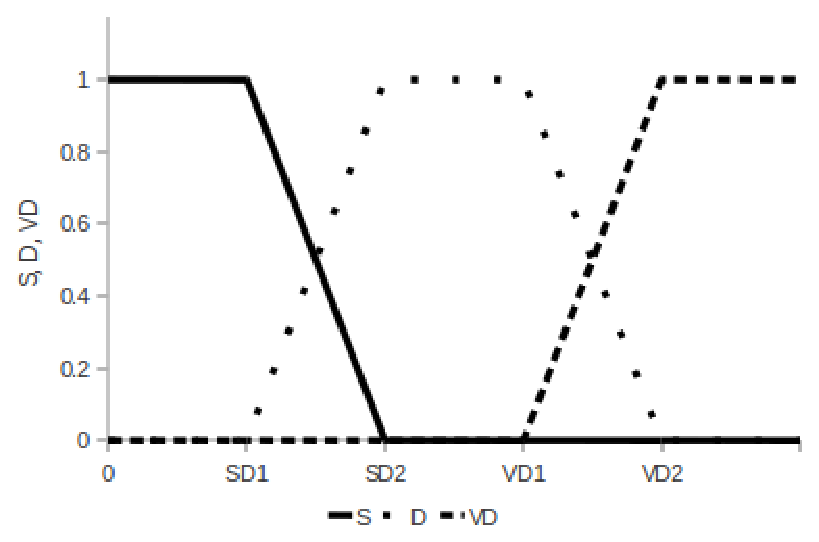
\includegraphics[height=0.42\linewidth]{similarity}
\begin{figure}[h!]
\label{fig:sim1}
\centerline{\psfig{figure=similarity.eps,width=0.5\textwidth}}
      \caption{Similarity}
\label{sim}
\end{figure}


\subsection{Context-aware ASM-based clustering}
\label{sec:contextaware}

The skeleton of this approach is based on the ASM-like algorithm from \cite{Chen04AnAdaptive} embellished with features from \cite{Chira07Stigmergic, Gaceanu10AnAdaptive, Schockaert04Fuzzy}. 
	
The agents decide upon the way they move on the grid based on their similarity with the neighbours, using fuzzy IF-THEN rules. Thus two agents can be similar (S), different (D), very different (VD). If two agents are similar or very similar they would get closer to each other. If they are different or very different they will get away from each other. The number of steps they do each time they move depend on the similarity level. So if the agents are $VD$ they would jump many steps away from each other; if they are $D$ they would jump less steps away from each other. In the end the ants which are $S$ will be in the same cluster. 
The similarity computation considers the actual structure of the data or the data density from the agent's neighbourhood; a bigger change from one agent to another translates into a certain similarity which then affects the agent's movement on the grid. 

Whenever it is supposed to make a move the agent can pro-actively decide to either move based on the similarity with its neighbours, like described above, or to move based on direct communication with other agents, located possibly outside its neighbourhood. 

The parameter $\alpha$ is the average distance  between agents and this changes at each step further influencing the fitness function. The parameter $\lambda$ influences the agents' activation pressure and it may decrease over time. The parameter $t$ is used for the  termination condition which could be something like \begin{math} t < t_{max}  \end{math}. The parameters $s_x, s_y$, the agent's vision limits may also be updated in some situations.  

\begin{algorithm}
\caption{Clustering}
\label{alg:clusteringcontext}
\begin{algorithmic}[1]
\STATE @ initialize parameters \begin{math}   \alpha, \lambda, t, s_x, s_y   \end{math}
	\FORALL {agent} 
		\STATE @ place agent at randomly selected site on the grid
	\ENDFOR
		\WHILE {not termination}
		\FORALL {agent} 
		\STATE @ compute agent’s fitness and activation probability $p_a$ according to Definition \ref{def:fitour} and 	Definition \ref{def:pa}
		\STATE r $\leftarrow$ random (0,1)
		\IF {$r < p_a$} 
			\STATE @ activate agent and adapatively move based on the context to a site in the neighbourhood using fuzzy IF-THEN rules
		\ELSE @ stay at current site and sleep
		\ENDIF
		\ENDFOR
		\STATE @ update parameters \begin{math}   \alpha, \lambda, t, s_x, s_y   \end{math}
	\ENDWHILE
	
\end{algorithmic}
\end{algorithm}

\begin{comment}
\begin{tabbing}
Algo\=rith\=m Clu\=ster\=ing is\\
	\>initialize parameters \begin{math}   \alpha, \lambda, t, s_x, s_y   \end{math}\\
	\>for \=each agent do\\
		\>\>place agent at randomly selected site on the grid\\
	\>endFor\\
	\>whil\=e (not termination)\\
		\>\>for each agent do\\
		\>\>\>compute agent’s fitness and activate probability $p_a$ according\\
		\>\>\>\>to definitions 5, 6 and 7\\
		\>\>\>r $\leftarrow$ random (0,1)\\
		\>\>\>if ($r < p_a$) then activate agent and adapatively move based \\  
						\>\>\>\> on the context to a site in the neighbourhood \\  
						\>\>\>\> using fuzzy IF-THEN rules\\
		\>\>\>else stay at current site and sleep\\
		\>\>\>endif\\
		\>\>endFor\\
		\>\>adaptively update parameters \begin{math}   \alpha, \lambda, t, s_x, s_y   \end{math}\\
	\>endWhile\\
endAlgorithm\\
\end{tabbing}
\end{comment}


%The entire clustering procedure can be best seen in figure ~\ref{fig:context} and will be detailed in the following.
%\begin{figure}[h!]
%  \centering
%  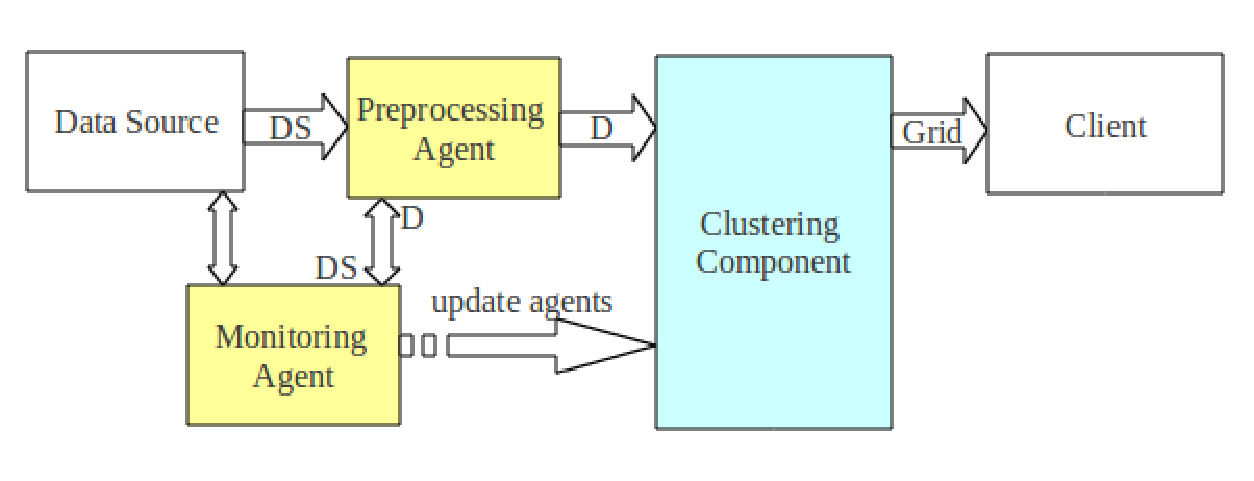
\includegraphics[width=0.75\textwidth]{context}
%  \caption{General overview of the clustering approach.
%}
%  \label{fig:context}
%\end{figure}

%\begin{figure}[h!]
%\centerline{\psfig{figure=context.eps,width=\textwidth}}
%      \caption{General overview of the clustering approach}
%\label{fig:context}
%\end{figure}


The approach from \cite{Chen04AnAdaptive} allows a high liberty to the ants' movements but only in their neighbourhood. The advantage of our approach is that it enables the  ants to communicate directly like in \cite{Chira07Stigmergic} therefore breaking the neighbourhood boundaries and thus decreasing the chance of ants to get trapped in local minima. The fuzzy IF-THEN rules governing the agents' movements are also allowing the agents to go beyond the neighbourhood limits; for example in the case of two very different ($VD$) agents it makes no point to keep them in a reachability distance; and it makes sense that two very different ($VD$) agents should move further away from each other than two different ($D$) agents do. Thus the system behaves more naturally. Compared to \cite{Gaceanu10AnAdaptive} the agents are able to adapt their movements if changes in the environment would occur which is an important feature in real-time systems, wireless sensor networks or data streams. As in any non-deterministic algorithm, the way of processing the data is not fixed. This leads to slightly different results from one execution to another as it will be seen i the experiments. However we should mention that our goal here is to obtain a certain quality of the clustering (a certain overall fitness of the agents), so it is unimportant for us which two items are misclassified. Another drawback of the approach is that there is an agent encapsulating every item being clustered. While this is an advantage compared to other methods, as shown in \cite{Chen04AnAdaptive}, we can imagine that in very large datasets the approach could become impractical in terms of memory consumption.

The algorithm we have presented is based on the adaptive ASM approach from \cite{Chen04AnAdaptive}. The major improvement is that, instead of moving the agents at a randomly selected site, we are letting the agents choose the best location. Agents can directly communicate with each other --- similar to the approach from \cite{Chira07Stigmergic}. In \cite{Schockaert04Fuzzy}, the fuzzy IF-THEN rules are used for deciding if the agents are picking up or dropping an item. In our model we are using the fuzzy rules for deciding upon the direction and length of the movement. Compared to \cite{Gaceanu10AnAdaptive} the agents are able to adapt their movements if changes in the environment would occur. 


\subsubsection{Methodology}
Let us consider the proposed clustering algorithm. Before it can be applied to cluster items in a given dataset, one needs to preprocess the data. 

The preprocessing phase is a process that is usually necessary and it takes place before any data mining operation. This preprocessing step is necessary because it is often the case that data comes from multiple heterogeneous sources which increases the chance of receiving low-quality data, i.e., noisy, missing or inconsistent data. 

Several data preprocessing techniques exist like data cleaning, data integration, data transformation and data reduction. Data cleaning involves transformations to correct wrong data and is used in general for removing noise and inconsistencies in data. Data integration is used for merging multiple sources of data into a single data store, such as a data warehouse while data transformations, like normalization can improve the accuracy and efficiency of the data mining algorithms that consider distance measurements. Data reduction leads to a reduced size of data by aggregating, eliminating redundant features, or clustering \cite{Han06DataMining}. Nevertheless, data preprocessing should be used with caution because it could destroy interesting features in data, maybe exactly what the data analyst is looking for. So from the above we only use data normalization for scaling the attributes in the range $[0, 1]$. Missing attributes values are filled in with $0$ so it could be considered that some data cleaning is also performed, but this would be all it is done in terms of destructive actions over the data. 

Normalization is particularly useful for algorithms like clustering because it helps preventing attributes with large ranges from outweighing attributes with smaller ranges. As a normalization method, the min-max normalization method is chosen because it preserves the relationships between the original data values as opposed to z-score normalization, and normalization by decimal scaling \cite{Han06DataMining}. 

For scaling the values in the $[0, 1]$ interval the following formula is used:

\begin{align}
A_{k} \leftarrow \frac{A_{k} - min_A}{max_A - min_A}, \forall k=\overline{1,\lvert A_{k} \rvert}, \exists i=\overline{1,\lvert \X \rvert}: A_{k} \in X_{i}
\end{align}
where $\X = \{X_i \vert i=\overline{1,\lvert \X \rvert}\}$ is the dataset with items to be clustered, $A_k$ denotes the value of the $k^{th}$ item in the considered attribute $A$, 
$min_A$ and $max_A$ are the minimum and, respectively, the maximum values over $A$.

The next step is to compute the disimilarity $\D$ between all items in the dataset $\X$:
\begin{align}
\D = \{d_{i,j} \vert i,j = \overline{1,\lvert \X \rvert}\}
\end{align}
where $d_{i,j}$ denotes the disimilarity between the items $X_i$ and $X_j$ from the dataset $\X$. The disimilarity $d_{i,j}$ between $X_i$ and $X_j$  could be the Euclidean distance between the two items:
\begin{align}
de (X_i, X_j) = \sqrt{\sum_{k=1}^{m}{(X_{i_k} - X_{j_k})^2} }
\end{align}
where $m = \lvert X_i \rvert = \lvert X_j \rvert$.

The disimilarity $\D$ between all items is sent to the clustering component. The clustering component first creates a grid according to the given definitions and then the population of ants is created, one ant for each data item. The process executes as described in the given algorithm leading to a clustering in data as explained. The grid containing the clustered data, i.e., ants can be sent to further components or can be visualized and interpreted by the data analyst.


\subsubsection{The advantages of the proposed approach}

The BM \cite{Deneubourg91TheDynamic} and LF \cite{Lumer94Diversity} models both separate ants from the objects being clustered, which increases computational cost. As noticed in \cite{Chen04AnAdaptive}, ants carrying isolated data items may fall into a infinite loop because they are unable to ever finding a proper location to drop down the isolated data items. This leads to an even higher computational time  consumption. The approach from \cite{Schockaert04Fuzzy} also keeps the ant and item to be clustered separated. The advantage of the ASM model is that ants directly represent the data items to be clustered. The ants move based on the similarity with the neighbouring fellows eventually forming distinctive groups and hence the corresponding data items are clustered. 
	
The approach from \cite{Chen04AnAdaptive} allows a high liberty to the ants' movements but only in their neighbourhood. The advantage of our approach is that it enables the  ants to communicate directly like in \cite{Chira07Stigmergic} therefore breaking the neighbourhood boundaries and thus decreasing the chance of ants to get trapped in local minima. The fuzzy IF-THEN rules governing the agents' movements are also allowing the agents to go beyond the neighbourhood limits; for example in the case of two very different ($VD$) agents it makes no point to keep them in a reachability distance; and it makes sense that two very different ($VD$) agents should move further away from each other than two different ($D$) agents do. Thus the system behaves more naturally, it becomes closer to human behaviour. Because, even if we are not aware of it, humans make decisions based on such if-then statements: if the weather is fine then I might go out, if the forecast for the weekend is bad weather then I will not plan a trip in the mountains. So if we want to have systems which mimic the human behaviour then fuzzy inference is a way towards this.

In the first model the agents represent the data items to be clustered and a change in the data item itself is not be handled at runtime. The extension to a context-aware dynamic system is be beneficial in many practical situations. 

In general, context-aware systems could greatly change the way we interact with the world — they could anticipate our needs and advice us when taking some decisions. In a changing environment context-awareness is undoubtly beneficial. The nowadays technology is able to support such systems --- devices with GPS are present in the lives of many of us. So a system can be aware about the location, it may know where the user is going, but  it could also be aware of the user's preferences or it could infer such preferences from a user's activity. Such systems could make much more relevant recommendations and support decision making. 

In the current approach each data item is encapsulated by an agent. While this is an advantage compared to the BM and LF models \cite{Deneubourg91TheDynamic,Lumer94Diversity} since it reduces computational cost, it also comes with a drawback: clearly if the data set has many items then the memory consumption is high.  An idea to overcome this issue would be to use a similar approach to the one from \cite{Karypis99Chameleon}. Here the clustering algorithm uses a sparse graph in which nodes represent data items  and edges have weights corresponding to similarities between data items. This representation enables Chameleon \cite{Karypis99Chameleon} to scale well and to successfully use datasets that are available in similarity space only  and not in metric spaces. 


\subsection{Case studies}
\label{sec:caseasm}

In this chapter computational experiments showing the potential of the proposed method are presented. In the first case study a custom dataset is considered and comparison with the k-means clustering is done suggesting the strength of the proposed algorithm. In the second case study the algorithm is tested on a larger dataset. Comments regarding the performance together with idea for further improvements are presented. The third case study is presenting a possible application of this clustering approach in a real-life scenario --- clustering web search results \cite{Gaceanu10AnAdaptive}.

\subsubsection{Synthetic dataset}

In order to evaluate the proposed algorithm the following custom dataset was considered:

\begin{tabular}{lllll}
\hline
\multicolumn{2}{c}{Test dataset} \\
\cline{1-5}
Id  & A1 & A2 & A3 & A4  \\ 
\hline
0 & 0.11 & 0.11 & 0.12 & 0.13\\
1 & 0.12 & 0.12 & 0.14 & 0.11\\
2 & 0.11 & 0.11 & 0.11 & 0.11\\
3 & 0.41 & 0.41 & 0.41 & 0.42\\
4 & 0.43 & 0.43 & 0.41 & 0.41\\
5 & 0.81 & 0.81 & 0.82 & 0.82\\
6 & 0.81 & 0.81 & 0.83 & 0.81\\
\hline
\end{tabular} 

\begin{align*}
\end{align*}
The algorithm was evaluated against this dataset and the following clusters were obtained:
\begin{itemize}
\item $Cluster0$ (0, 1, 2)
\item $Cluster1$ (3, 4) 
\item $Cluster2$ (5, 6). 
\end{itemize}

In Figure \ref{testDs_grid} the final position of the agents can be seen. The agents are labelled with values from $0$ to $6$, $-1$ denotes and empty position.
%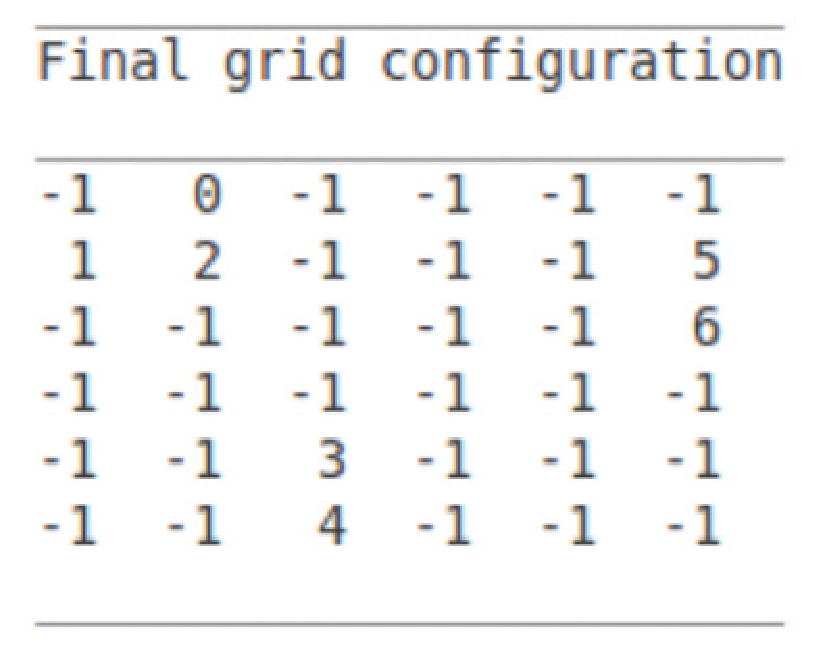
\includegraphics[scale=0.75]{testDs_grid}
\begin{figure}[h!]
\centerline{\psfig{figure=testDs_grid.eps,width=0.3\textwidth}}
      \caption{Final grid configuration - synthetic dataset}
\label{testDs_grid}
\end{figure}


In Figure \ref{testDs_membership} one can see the membership degree of each agent to each cluster. In this test case, because the points from different clusters are very well separated, the membership degree of each ant to the clusters is either $0$ or $1$. Of course in reality it is not always the case to have so clearly separated points to cluster and in such cases the membership degrees of the points will belong to the interval $[0, 1]$ as opposed of belonging to the set $\{0, 1\}$.
%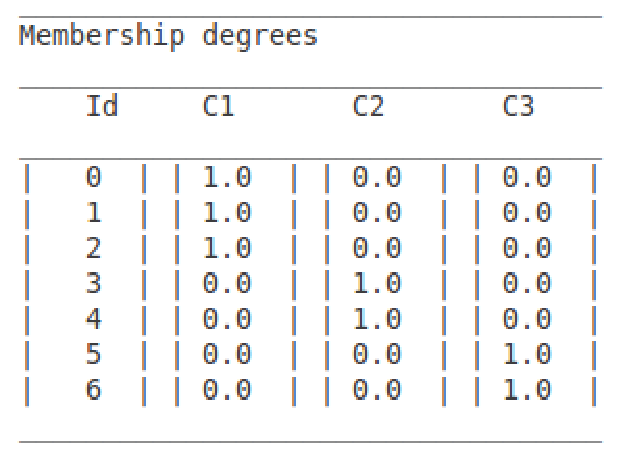
\includegraphics[scale=0.75]{testDs_membership}
\begin{figure}[h!]
\centerline{\psfig{figure=testDs_membership.eps,width=0.3\textwidth}}
      \caption{Membership degrees - synthetic dataset}
\label{testDs_membership}
\end{figure}

In Figure \ref{weka_customds} the reported result from Weka \cite{Hall09Weka} on the same dataset is shown.  As it will be seen the k-means algorithm has 3 misclassifications while our algorithm has no misclassifications in this test case. Further comments are superfluous for this test case.

%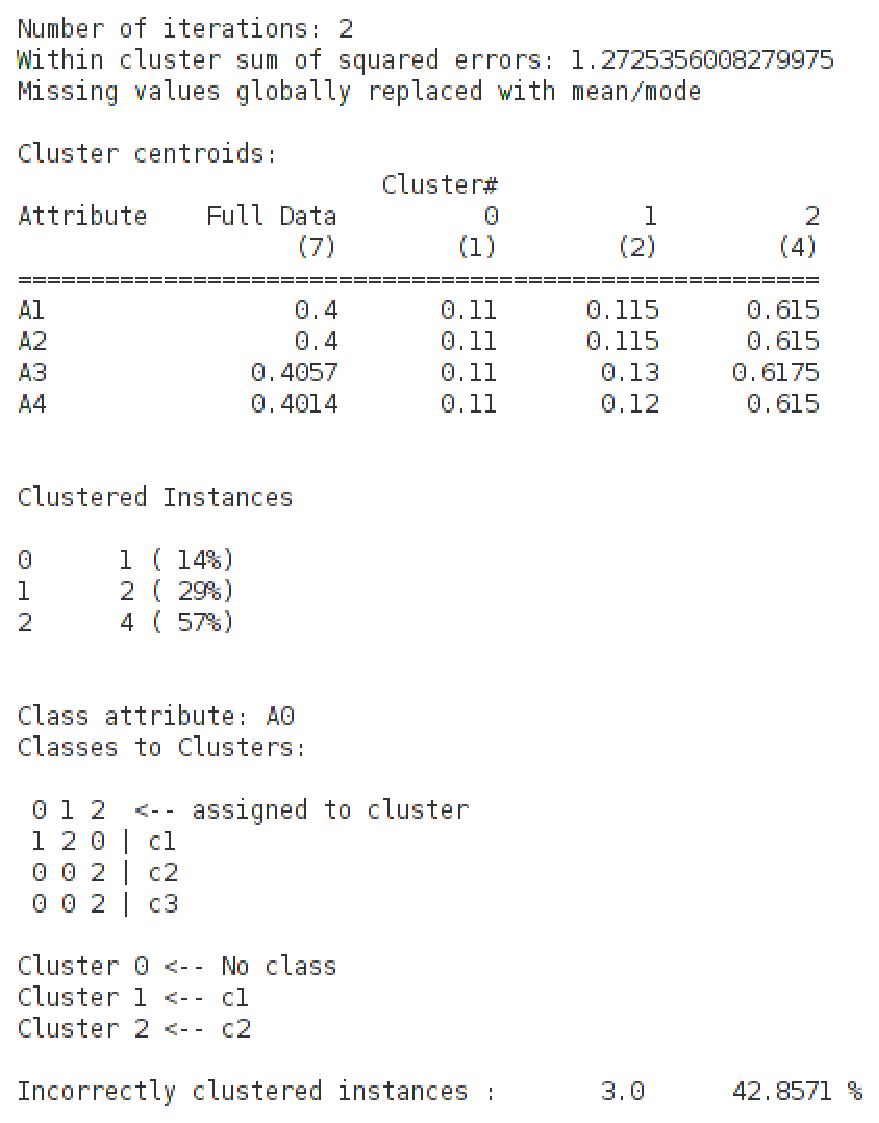
\includegraphics[scale=0.75]{weka_customds}
\begin{figure}[h!]
\centerline{\psfig{figure=weka_customds.eps,width=0.75\textwidth}}
      \caption{Classical approach result - synthetic dataset}
\label{weka_customds}
\end{figure}

\subsubsection{Iris dataset}

In order to test the algorithm in a real-world scenario, the Iris dataset was considered \cite{website:iris}. The data set contains three classes of $50$ instances each, each class referring to a type of iris plant. There are four attributes plus the class: sepal length in $cm$, sepal width in $cm$, petal length in $cm$, petal width in $cm$, class (Iris Setosa, Iris Versicolour, Iris Virginica). This dataset is appropriate for rather testing classification, but it was preferred for clustering too because the class attribute is given and hence there a way to evaluate the algorithm. So apparently it would be ideal for the algorithm to produce three clusters of $50$ instances, the three clusters corresponding to the given three classes. 

The last two attributes (petal length in cm and petal width in $cm$) are highly correlated according to \cite{website:iris}. We do not dismiss any of these attributes though  because as explained in the methodology we would like to keep as much of the data unchanged. We do however scale the data to the interval $[0, 1]$. At this point the clustering process can be started as described in the corresponding section and a result is given. In the final grid configuration (Figure \ref{iris_grid}) some columns from the middle, where a bigger space can be seen, have been removed in order for the grid to fit into the page.

%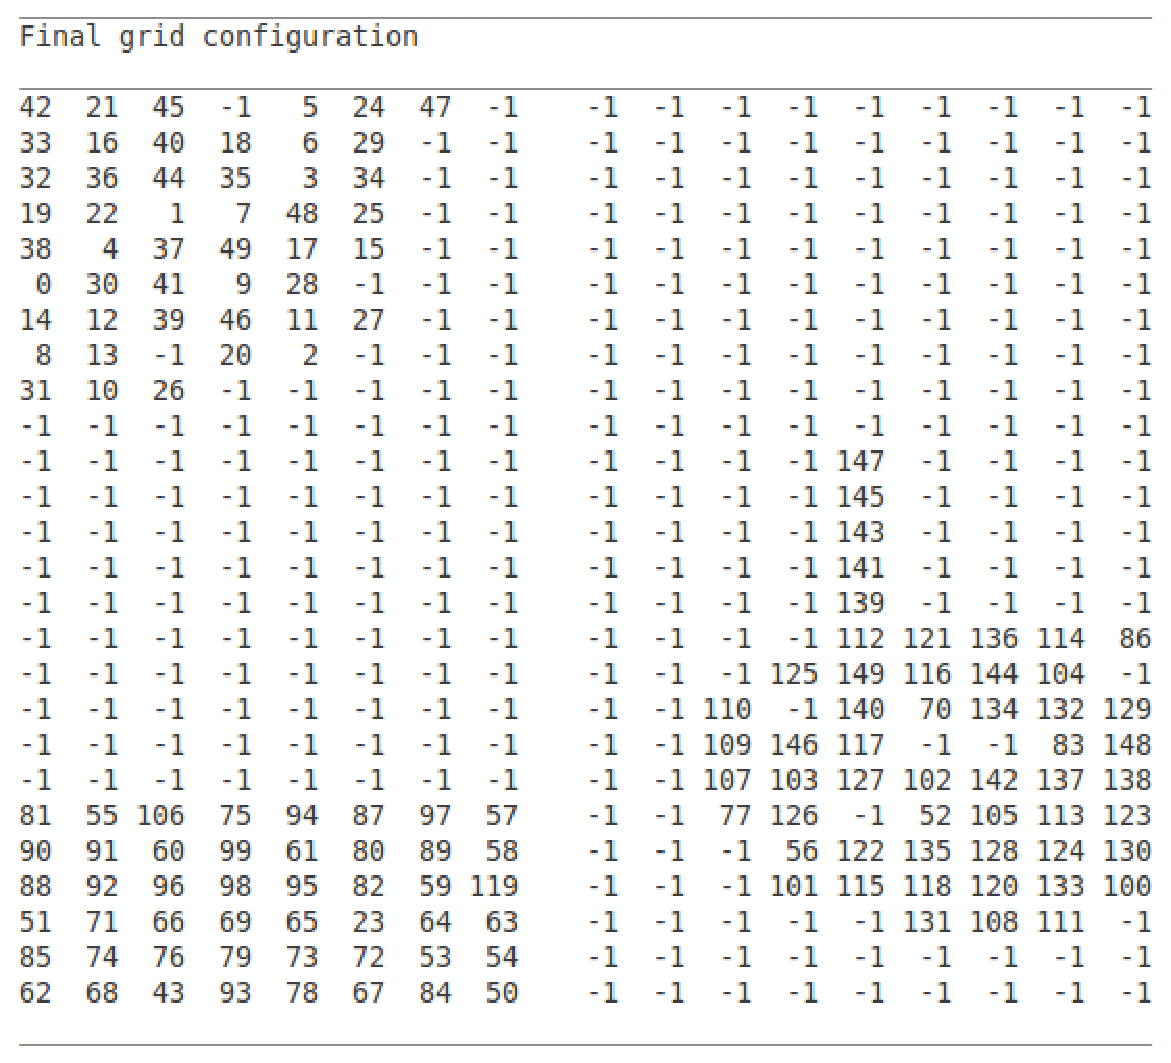
\includegraphics[scale=0.75]{iris_grid}
\begin{figure}[h!]
\centerline{\psfig{figure=iris_grid.eps,width=\textwidth}}
      \caption{Final grid configuration - Iris dataset}
\label{iris_grid}
\end{figure}


As it can be seen from Figure \ref{iris_grid}, all the agents have been assigned to clusters. As it will be seen in Figure \ref{iris_membership} they actually belong to the clusters in a certain degree.

%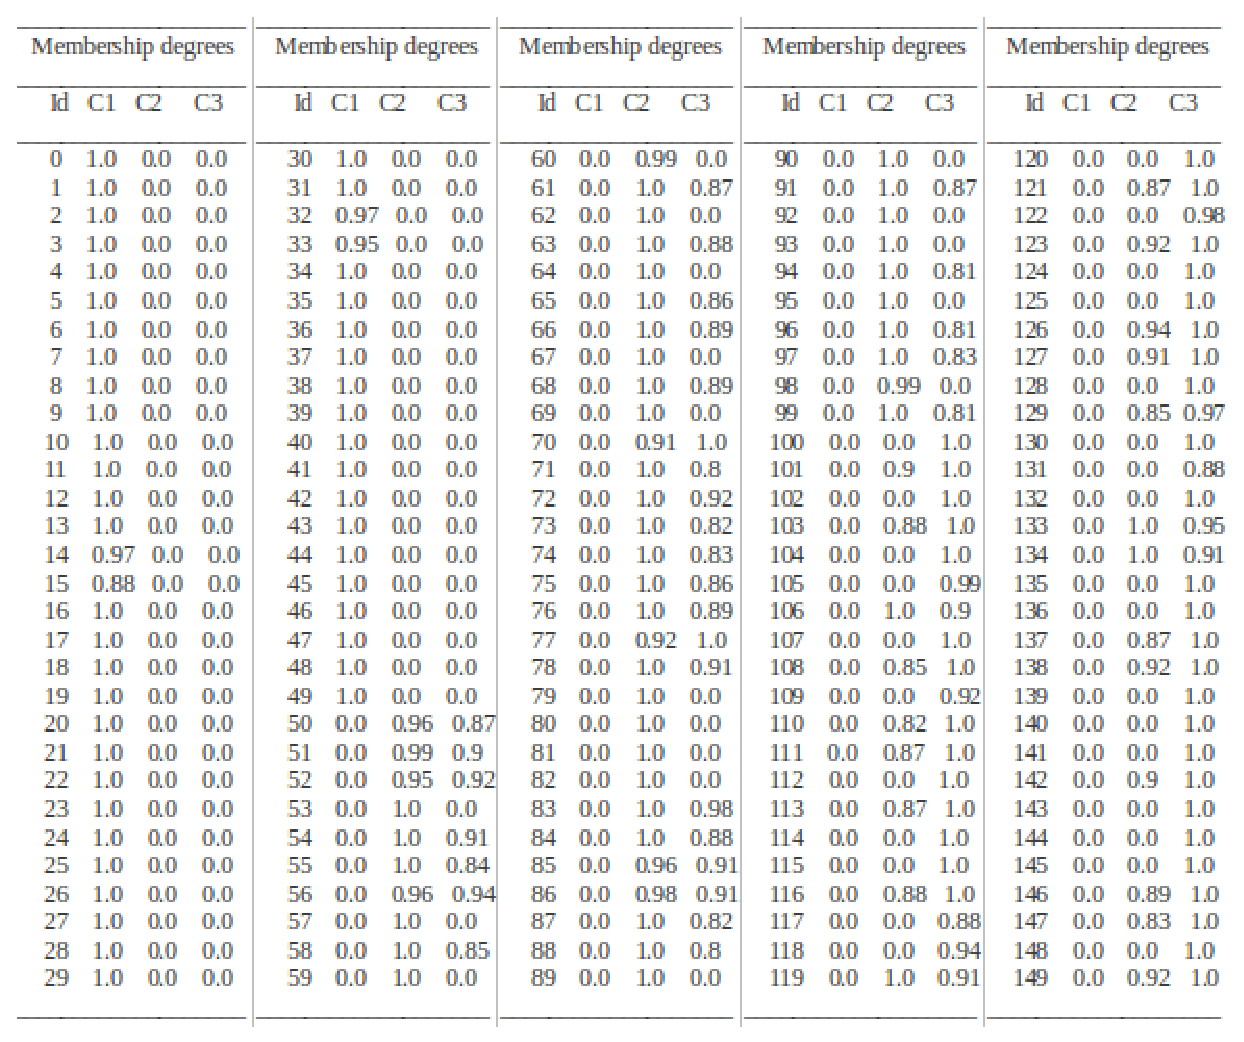
\includegraphics[scale=0.75]{iris_membership}
\begin{figure}[h!]
\centerline{\psfig{figure=iris_membership.eps,width=\textwidth}}
      \caption{Membership degrees - Iris dataset}
\label{iris_membership}
\end{figure}


According to the Iris dataset \cite{website:iris}, items ranging from $0$ to $49$ belong to the first class, items ranging from $50$ to $99$ belong to the second class and items ranging from $100$ to $149$ belong to the third class. So from the grid table it appears that the following clusters contain some misclassifications:
\begin{itemize}
\item $Cluster1$ (items $0$ -- $49$): no misclassifications
\item $Cluster2$ (items $50$ -- $99$): 106, 119, 23, 43
\item $Cluster3$ (items $100$ -- $149$): 86, 70, 83, 52, 56
\end{itemize}
So it appears that the algorithm has misclassified $9$ items. 

Let us check each item in more detail. In order to do this deeper analysis we first need a representative for each cluster. We try to simulate the real-life process in which the data analyst would point such representatives with the mouse. Of course that if he deals with a high density cluster then he normally can only make a rough approximation. We can refine his choice by proposing an item in the neighbourhood which has the highest fitness. So what we do in this test is to randomly choose a candidate representative from each cluster and then replace him with the best fitted agent from a certain radius; a radius $r=2$ was considered for this case study.
The agents $34$, $90$, $120$ resulted from this process as final representatives for clusters $1$, $2$ and $3$ respectively.

In the following the similarity between each of the above reported misclassification and the corresponding representative is given. The membership degree to each cluster is also considered. As in the first test case, the Euclidean distance between items has been used as a similarity metric. So a small similarity value i.e. distance between two items means that the two items are similar, should stay together.\\

\begin{tabular}{lllll}
\hline
\multicolumn{2}{c}{Cluster2 --- RepresentativeId (90)} \\
\cline{1-5}
MisclassificationId & Similarity  & C1 & C2 & C3\\ 
\hline
106 & 0.20 & 0.0 & 1.0 & 0.9\\
119 & 0.18 & 0.0  &  1.0 &   0.91\\
23 & 0.50 & 1.0 &   0.0 &   0.0\\
43 & 0.51 & 1.0 &   0.0 &   0.0\\
\hline \\
\end{tabular} 


From the table Cluster2 --- RepresentativeId (90) it can be seen  that items $23$ and $43$ are clearly miclassifications. Both of them should surely belong to $Cluster1$ as they have a membership degree of $1$ to this cluster and $0$ to the other clusters. Moreover, their similarity value of $0.50$ and $0.51$ respectively to the representative item $90$ should have made these agents to reject each other; because such similarity values would  make them $D$ ($Different$) in terms of the considered fuzzy  sets. The considered limit values for the fuzzy sets described in a previous section are: $SD1(0.2), SD2(0.4), VD1(0.6), VD2(0.7)$.

On the other hand, it is unclear why should items $106$ and $119$ be considered misclassifications. According to our similarity measures they have a $0.20$ and a $0.18$ similarity with the representative item $20$. This makes them $S$ ($Similar$) with this item. The membership degree with $Cluster2$ suggests that these items belong in this cluster. However the membership degree with $Cluster3$ is also high. The highest membership degree is with $Cluster2$ though and because of this it could be claimed that the items are actually correctly classified with respect to the considered metric. However we believe that items $106$ and $119$ cannot be considered to strictly belong either $Cluster2$ or $Cluster3$ as they are clearly at the border of the two clusters so they belong to both. In this case we also believe that they should not be regarded as misclassifications. \\

\begin{tabular}{lllll}
\hline
\multicolumn{2}{c}{Cluster3 --- RepresentativeId (120)} \\
\cline{1-5}
MisclassificationId & Similarity   & C1 & C2 & C3\\ 
\hline
86 & 0.34 & 0.0 &    0.98 &   0.91\\
70 & 0.26  & 0.0 &   0.91 &  1.0\\
83 & 0.32 & 0.0 &  1.0 &  0.98\\
52 & 0.32 & 0.0 &   0.95 &  0.92\\
56 & 0.31 & 0.0 &   0.96 &  0.94\\
\hline\\
\end{tabular} 

Like items $106$ and $119$, the items from the table Cluster3 --- RepresentativeId (120) should also not count as misclassifications for the same reasons from above. This leaves only items $23$ and $43$ as misclassifications.

A final remark regarding the membership degrees table. It may be observed that starting with item $50$ a lot of instances have high membership degrees to both $Cluster2$ and $Cluster3$. This suggests that the  members of these two classes are not linearly separable as mentioned in \cite{website:iris} so a clustering process could also merge these two clusters and hence report only two clusters instead of three. 

In Figure \ref{weka_iris} we will list the output of the k-means clustering algorithm of the Iris dataset \cite{website:iris} from Weka \cite{Hall09Weka}. As it can be seen, $17$ instances are reported as misclassified so our proposed model delivers better results than k-means for a real-world dataset.

%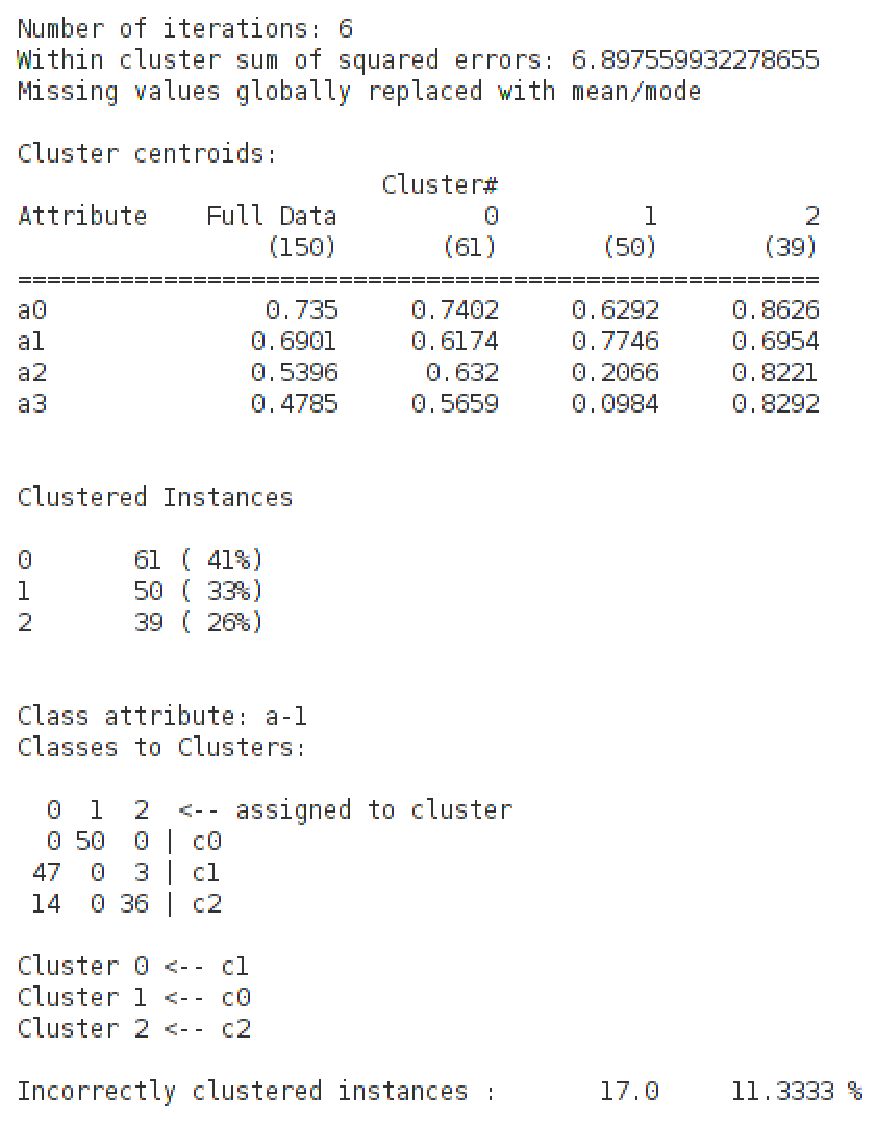
\includegraphics[scale=0.75]{weka_iris}
\begin{figure}[h!]
\centerline{\psfig{figure=weka_iris.eps,width=0.75\textwidth}}
      \caption{Classical approach result --- Iris dataset}
\label{weka_iris}
\end{figure}


A final remark regarding the membership degrees table. It may be observed that starting with item $50$ a lot of instances have high membership degrees to both $Cluster2$ and $Cluster3$. This suggests that the  members of these two classes are not linearly separable as mentioned in \cite{website:iris} so a clustering process could also merge these two clusters and hence report only two clusters instead of three. 


\subsubsection{Clustering web search results}
This case study was presented in \cite{Gaceanu10AnAdaptive}. An initial version of the clustering algorithm presented here was applied for clustering web search results showing the applicability in real life of this research. In general, web search engines respond to queries by returning a list of links to web pages that are considered relevant. These queries are often ambiguous or too general for accurately expressing the user’s information need. Thus most of the search results are not really relevant. So users are often browsing through a long list of items in order to find what they are actually looking for. And hence the idea to cluster web search results so that the output would be a list of labelled clusters. 

In the other test case the Euclidean distance was used to measure the (di)similarity between items. In this test case the following formula is used:
\begin{align}
\label{rel:tfidf}
tfidf_{t,d}=tf_{t,d} \cdot idf_t\
\end{align}
\begin{align}
\label{rel:idf}
idf_t=log\frac{N}{df_t}
\end{align}
where $N$ is the total number of documents in the collection, \begin{math} df_t  \end{math} (document frequency) is the number of documents in the collection containing the term $t$.
Thus the $idf$ (inverse document frequency) of a seldom term is high, while as the $idf$ of an often term is low.
So, $tfidf$ (term frequency inverse document frequency) assigns to term $t$ a weight in document $d$ that is:
\begin{itemize}
\item  highest when given a small number of documents, $t$ has many occurrences within them
\item  lower when either given a document $d$, the term $t$ occurs few times or when it occurs in many documents
\item  lowest when $t$ occurs in almost all documents.
\end{itemize}
So documents may be seen as a vector of components corresponding to each term in the dictionary, together with the associated weight (given by $tfidf$). This weight is equal to zero for dictionary terms that do not appear in the document.

In order to evaluate the algorithm for clustering web search results \cite{Gaceanu10AnAdaptive} we have made a Java application containing the following module: a web crawler, a weighing module and a clustering module. 

The Web crawler browses the World Wide Web in a methodical, automated manner with the purpose of parsing and indexing the HTML pages. To explore the Web graph the breadth-first
algorithm is used. The crawler receives as input a set of starting pages and it extracts the text and the links. 	
The weighting component has two parts: a $MySQL$ procedure and a Java thread that executes the procedure at a given interval of time. Using the formulas from relations (\ref{rel:tfidf}) and (\ref{rel:idf}) we apply a stored procedure to update the token's weights. When performing a normal search, the dot product between the query vector and documents from the index is computed and the documents are returned in decreasing order.
A matrix of document similarities is given to the clustering component. The clustering component uses the Algorithm \ref{alg:fuzzyasmclustering} and outputs the clusters and the document ids from each cluster. For example, suppose we are searching for the word ``mouse''. We take only the first $5$ search results and send them to the clustering component:

\begin{table}[ht] 
\caption{First 5 search results} % title of Table 
\centering % used for centering table 
\begin{tabular}{cc} % centered columns (3 columns) 
\hline\hline %inserts double horizontal lines 
Document id  & Site  \\ [0.5ex] % inserts table %heading 
\hline % inserts single horizontal line 
0 & http://computer.howstuffworks.com/mouse.htm \\ % inserting body of the table
1 & http://en.wikipedia.org/wiki/Mouse \\
2 & http://www.newegg.com/ \\
3 & http://animal.discovery.com/  \\
4 & http://computer.howstuffworks.com/share-redirect? \\
& type=facebook\&cid=1106  \\ 

\hline %inserts single line 
\end{tabular} 
\label{table:nonlin} % is used to refer this table in the text 
\end{table}

The clustering component will output the following clusters:
\begin{itemize}
	\item 	Cluster0: 0, 2, 4 
	\item Cluster1: 1, 3.
\end{itemize}

This result was found after $46$ iterations (the grid configuration has stabilized) and the computation took less than $1$ second. We have used the following initial values for the 
parameters:  \begin{math} s_x = s_y =  \lambda = 2 \end{math}. The value of the parameter \begin{math} \alpha \end{math} is computed according to relation (\ref{rel:alpha1}).  The parameter $t$ is used for the  termination condition. In our approach the termination condition is simply  \begin{math} t < t_{max}  \end{math} and we have considered  \begin{math} t_{max} = 100 \end{math}, i.e., the algorithm iterates $100$ times.
If we look at the first cluster, we see that we have documents containing information about the ``mouse'' from computing and if we look at the second cluster we see that we have documents containing information about ``mouse'' --- the animal. So one would have the possibility to browse through the desired cluster of search results only. We consider that this is a good example for showing the applicability of our methods in real life.

\subsection{Discussion}
\label{sec:clustdiscussion}

The BM \cite{Deneubourg91TheDynamic} and LF \cite{Lumer94Diversity} models both separate ants from the objects being clustered, which increases computational cost, as noticed in \cite{Chen04AnAdaptive}. Also the following unfortunate situation could occur: ants which carry isolated data items may get trapped into infinite loops since they will never find a proper location to drop down the isolated data items which will lead to a higher amount of computational time consumption. The advantage of the ASM model is that ants directly represent the objects to be clustered. The results reported in \cite{Chen04AnAdaptive} show that the LF model needs one million iterations in order to achieve satisfying results, while the ASM model  needs five thousand iterations. By using direct communication and fuzzy if-then rules we have managed to reduce the number of necessary iterations from the order of thousands to the order of hundreds. As being still in an experimental phase, there is a penalty at the level of each iteration for the moment, but further work is continuously done in order to improve this aspect. 

The approach from \cite{Schockaert04Fuzzy} keeps the ant and item to be clustered separated and the behaviour of the artificial ants is governed by fuzzy if-rules --- in their approach the rules are used in deciding weather or not to pick-up an item as opposed to our approach where the fuzzy rules are governing the movement strategy of each individual ant. In order to evaluate the algorithm they define a classification error which strongly penalizes a  solution in which a wrong number of clusters has been obtained. The results are provided in terms of the classification error defined there and they were found after one million iterations. Also, unlike our approach, they consider each item as uniquely belonging to a cluster which, as we have seen in the second case study, is in our opinion not the best approach. 

So by using direct communication and fuzzy if-then rules we have managed to significantly improve the number of necessary iterations. An important achievement over the considered approaches are the use fuzzy memberships because they allow us to have a better view over the data. As we have seen along the case studies, this is especially important when dealing with non-linearly separable classes where we can spot items belonging in a high degree to both classes avoiding wrong classifications or misjudgements over such items. This makes our method more robust than the considered approaches. 

The approach from \cite{Chen04AnAdaptive} allows a high liberty to the ants' movements but only in their neighbourhood. The advantage of our approach is that it enables the  ants to communicate directly like in \cite{Chira07Stigmergic} therefore breaking the neighbourhood boundaries and thus decreasing the chance of ants to get trapped in local minima. The fuzzy IF-THEN rules governing the agents' movements are also allowing the agents to go beyond the neighbourhood limits; for example in the case of two very different ($VD$) agents it makes no point to keep them in a reachability distance; and it makes sense that two very different ($VD$) agents should move further away from each other than two different ($D$) agents do. Thus the system behaves more naturally. Compared to \cite{Gaceanu10AnAdaptive} the agents are able to adapt their movements if changes in the environment would occur which is an important feature in real-time systems, wireless sensor networks or data streams. As in any non-deterministic algorithm, the way of processing the data is not fixed. This leads to slightly different results from one execution to another --- for example in our experiment we had two misclassifications, namely items $23$ and $43$, but at another execution some other items could be misclassified. However we should mention that our goal here is to obtain a certain quality of the clustering (a certain overall fitness of the agents), so it is unimportant for us which two items are misclassified. Another drawback of the approach is that there is an agent for each item being clustered. While this is an advantage compared to other methods, as shown in \cite{Chen04AnAdaptive}, we can imagine that in very large datasets the approach could become impractical in terms of memory consumption.

\section{Incremental clustering}
\label{chap:incrementalclustering}

The idea behind incremental clustering is that it is possible to consider one instance at a time and assign it to existing clusters without significantly affecting the already existing structures. This chapter presents an incremental clustering approach based on ASM.

\subsection{General considerations}

The idea behind incremental clustering is that it is possible to consider one instance at a time and assign it to existing clusters without significantly affecting the already existing structures. The incremental approach to clustering is also applicable in online situations like wireless sensor networks or data streams. Ongoing research is done in the area sensor data and data stream mining \cite{Spinosa09Novelty,Haghighi09Context,George09Spatio}. In \cite{Spinosa09Novelty}, a new approach to novelty detection in data streams is presented. The ability to detect new concepts is an important aspect in machine learning systems. The approach presented in this paper \cite{Spinosa09Novelty} takes novelty detection beyond one-class classification, by detecting emerging cohesive and representative clusters of examples, and then further by merging similar concepts. The proposed method goes in the direction of constructing a class structure that aims at reproducing the real one in an unsupervised continuous learning fashion. The paper \cite{Haghighi09Context} presents a general approach for context-aware adaptive mining of data streams that tries to dynamically and autonomously adjust data stream mining parameters according to changes in context and situations. Data stream processing adaptation to variations of data rates and resource availability is crucial for consistency and continuity of running applications like health care systems.  In \cite{George09Spatio} a new data model called Spatio-Temporal Sensor Graphs (STSG), which is designed to model sensor data on a graph by allowing the edges and nodes to be modelled as time series of measurement data is presented. It is shown how this model could be applied in finding patterns like growing hotspots in sensor data. The case studies and the related study show that the presented model is less memory expensive. 

In incremental clustering only the cluster representations need to be kept in memory so not the entire dataset and thus the space requirements for such an algorithm are very small. Whenever a new instance is considered an incremental clustering algorithm would basically try to assign it to one of the already exiting clusters. Such a process is not very complex and therefore the time requirements for an incremental clustering algorithm are also small.

In \cite{Gaceanu11AContext}, the clustering problem is approached by the idea of context-aware ASM agents. The agents are able to detect changes in the environment and adjust their moves accordingly. Unlike the agents from the classical ASM model \cite{Chen04AnAdaptive} the agents from \cite{Gaceanu11AContext}  are able to communicate directly therefore breaking the neighbourhood boundaries and thus decreasing the chance of ants to get trapped in local minima. The agents are able to adapt their movements if changes in the environment would occur. However only changes in the features of already existing data items are handled. So clustering new incoming data items is not an issues in the approach from \cite{Gaceanu11AContext}. In this sense the incremental approach from this paper represents a natural step forward.

In \cite{Goyal} an interesting incremental clustering approach is presented similar to the incremental DBSCAN algorithm \cite{DBSCANIncremental}. In the incremental version of the  DBSCAN clustering algorithm data items can be added to existing clusters, one item at a time. The main difference of the approach from \cite{Goyal} is that it adds groups of items to existing clusters. The data points to be added are initially clustered using the DBSCAN algorithm \cite{DBSCAN} and the resulted clusters are merged with already existing ones. In other words, instead of adding data items incrementally the algorithm is adding clusters incrementally. 

Kamble uses in \cite{Kamble} a genetic algorithm for incrementally cluster data. The genetic algorithm \cite{Genetic} uses and manipulates a population of potential solutions in the attempt to obtain the optimal solutions and a generation is completed when every individual from the population has performed the genetic operators. The individuals from the resulted population will be better fitted with respect to the objective function. The algorithm from \cite{Kamble} works in metric spaces and it is a density-based approach as the key idea is that for each element of a cluster the number of items in the neighbourhood need to be above a certain threshold.

Lee et al. present in \cite{Lee02Inc} a method to implicitly resolve ambiguities using an incremental clustering in Korean to English cross language information retrieval. In their approach a query in Korean is first translated into English using a Korean-English dictionary and then documents are retrieved for the translated query terms. Query-oriented document clusters are incrementally created for the top ranked retrieved documents and the weight of each retrieved document is recomputed based on the created clusters. Considering their experiments the authors conclude that their method outperforms the monolingual retrieval.

In \cite{Charikar97Inc} an incremental clustering model is considered where the goal is to efficiently attempt to maintain clusters of small diameter as new items to be clustered are arriving. The dual clustering problem where clusters have a fixed diameter and the goal is to minimize the number of clusters is also considered. The authors focus their study in performing detailed running time complexity analysis of their approach compared to greedy algorithms and  to static clustering approaches. 

In \cite{Li10Incclust} an incremental clustering for trajectories is presented. Due to their sequential nature, trajectory data (or moving objects) are often received incrementally as flows of data from various possible sources like GPS. Most of the existing trajectory clustering algorithms are developed for static datasets, but, as the authors remark, such static approach are not suitable when frequent reclustering is needed and when  huge amounts of trajectory data are  accumulated constantly and needs immediate processing.
The proposed incremental approach contains two parts: an online micro-cluster maintenance and an offline macro-cluster
creation. Authors explain that micro-clusters are used to store compact summaries of similar trajectory line segments, which take much smaller space than raw trajectories. Incremental online update takes place on micro-clusters. Then 
macro-clustering is performed on the set of micro-clusters. Authors argue that since the number of micro-clusters is smaller than that of original trajectories, the macro-clusters generation is efficient. 

In \cite{Li11Training} a method for training set compression by using incremental clustering is proposed. 
The size of the training set can greatly influence the performance of a classifier because it is difficult to be stored in memory and to process it. So reducing the size of a training set is undoubtedly beneficial for a classification process. 
Training set compression is a method for reducing the size of the training set without having a negative impact on the classification accuracy. It attempts to eliminate redundancy in a dataset. Sequential leader clustering \cite{Hartigan75Clustering} is a classical clustering algorithm that may be used to eliminate redundancy. The samples to be discarded are considered redundant if they are close to one of the samples in the clusters. Hence the process of clustering may also be viewed as a subsampling process because clustering guarantees that all the samples in a group are separated at a certain  distance which is greater than a minimal threshold and in the approach from \cite{Li11Training}, this subsampling based compression is introduced.

Our incremental clustering approach is based on the ASM-like algorithm from \cite{Chen04AnAdaptive}. In the ASM model, due to the need for security, the ants are constantly choosing a more comfortable environment to sleep in. The ants feel comfortable among individuals having similar characteristics. In ASM, each data item is represented by an agent, and his purpose is to search for a comfortable position for sleeping in his surrounding environment. While he doesn't find a suitable position to have a rest, he will actively move around to search for it and stop when he finds one; when he is not satisfied with his current position, he becomes active again. 

If the fitness is low then the probability of activation is high so the agent is probably going to wake up, move and search for a better place to sleep. Conversely if the fitness is high then the probability is low so most probably the agent will stay and sleep.

\subsection{Incremental ASM approach}

At the beginning of the algorithm from \cite{Chen04AnAdaptive}, the agents are randomly scattered on the grid in active state. They randomly move on the grid.
In each loop, after the agent moves to a new position, it will recalculate its current fitness $f$ and probability $p_a$ so as to decide whether it needs to continue moving. The same $p_a$ as in \cite{Chen04AnAdaptive} is used:

\begin{definition}
The activation probability of $agent_{i}$ is:
\begin{align} 
p_a(agent_i)=cos^\lambda (\frac{\pi}{2}f(agent_i))
\end{align}
\end{definition}

\begin{remark}
If the current $p_a$ is small, the agent has a lower probability of continuing to move on the grid and higher probability of stopping at the current location and taking a rest. Otherwise the agent will stay in active state and continue moving. The agent's fitness is related to its similarity with other agents in its neighbourhood. 
\end{remark}

\begin{remark}
For computing the fitness the Definition \ref{def:fitour} is used.
\end{remark}

With increasing number of iterations, such movements gradually increase, eventually, making similar agents gathered within a small area and different types of agents located in separated areas. Thus, the corresponding data items are clustered.

\begin{comment}
\begin{definition}
%\textbf{Definition 6.}\\
The agent fitness is defined as follows:
\begin{align} 
f(agent_i)=\frac{1}{v} \sum_{a_j \epsilon N(a_i)} \frac{\alpha^2}{\alpha^2+ disim(a_i,a_j)de(a_i,a_j)},\\
 \end{align}
\begin{align}
v=\frac{1}{(2s_x + 1) (2s_y + 1)}
\end{align}
\begin{align}
\alpha=\frac{1}{n(n-1)} \sum_{i=1}^{n} \sum_{j=1}^{n} de(a_i,a_j),
\end{align}  
 where:
 \begin{itemize}
\item   $a_i$ and $a_j$ respectively denote $agent_i$ and $agent_j$,
\item $de(a_i,a_j) $  represents the Euclidean distance between the agents on the grid,
\item $disim(a_i,a_j)$  denotes the dissimilarity between the two agents. 
\end{itemize}
\end{definition}
\end{comment}
	
A high level pseudo-code of our incremental clustering algorithm is presented in Algorithm \ref{alg:clusteringinc}.
 

\begin{algorithm}
\caption{Algorithm clustering}
\label{alg:clusteringinc}
\begin{algorithmic}[1]

\STATE @ initialize parameters \begin{math}   \alpha, \lambda, t, s_x, s_y   \end{math}
\STATE @  initialize an agent $a_0$ for the first arrived item and create a cluster $c_0$ containing agent $a_0$
	\WHILE {condition}
	\FORALL {item i} 
	\STATE @ create an agent $a_i$ and randomly place it on the grid
	\STATE  j $\leftarrow$ random\{0, i\}
	\IF {$isSimilar(a_i, a_j)$}

	\STATE  $groupSimilar(a_i, a_j)$
	\ELSE 
	\STATE  $add(U, a_i)$	// U --- the set of unclustered agents
	\ENDIF
	\IF {$hasElements(U)$}
	\STATE   	$a_{asm} \leftarrow getRandomAgent(U)$
	\STATE  $tryActivate(a_{asm})$
	\ENDIF
	\ENDFOR
	\STATE @ adaptively update parameters
	\ENDWHILE

\end{algorithmic}
\end{algorithm}

\begin{comment}
\begin{tabbing}
Algo\=rith\=m Clu\=ster\=ing is\\
	\> initialize parameters \begin{math}   \alpha, \lambda, t, s_x, s_y   \end{math}\\
	\> initialize an agent $a_0$ for the first arrived item and\\
	\>\> create a cluster $c_0$ containing agent $a_0$\\
	\> while (condition)\\
	\>\> for each item i \\
	\>\>\> create an agent $a_i$ and randomly place it on the grid\\
	\>\>\> j $\leftarrow$ random\{0, i\}\\
	\>\>\> if $isSimilar(a_i, a_j)$\\
	\>\>\> then \\
	\>\>\>\> 	$groupSimilar(a_i, a_j)$\\
	\>\>\> 	else\\ 
	\>\>\>\> 	$add(U, a_i)$	// U --- the set of unclustered agents\\
	\>\>\> endif\\
	\>\>\> if $hasElements(U)$\\
	\>\>\> then \\
	\>\>\>\> 	$a_{asm} \leftarrow getRandomAgent(U)$\\
	\>\>\>\>	$tryActivate(a_{asm})$\\
	\>\>\> endif\\
	\>\> endfor\\
	\>\> adaptively update parameters\\
	\> endwhile\\
endAlgorithm\\
\end{tabbing}
\end{comment}

The algorithm continuously receives new items to be clustered. For the first such item, a new agent is created that encapsulates this item. As in the classical ASM model, one agent per item will be allocated. A new cluster is created (the first one) and the agent is added to this cluster. In the following, whenever a new item $i$ arrives, a new agent, $a_i$, is created. This agent is randomly placed on the grid and contacts an already existing agent from the grid. If they are similar then they are grouped together otherwise the agent $a_i$ is added to the set of unclustered agents, $U$. The $groupSimilar(a_i, a_j)$ procedure groups together two agents, i.e., the agent $a_i$ moves towards the agent $a_j$ on the grid and also it is added to the $a_j$'s cluster. If $a_j$ is not already in a cluster then a new cluster containing both agents is created. Whenever a new cluster is created we try to merge it with an already existing cluster. The merging is performed based on the similarity between the cluster representatives. The representative of a cluster is either the first item that was added to the cluster or an item pointed out, i.e., manually chosen by the data analyst. The similarity between two agents will be discussed immediately. To the cluster representatives we will come back in the experiments section.

In the final step of the for loop we test if the set of unclustered agents is not empty and if it contains elements then we try to activate a randomly extracted agent from there. In $tryActivate(a_{asm})$ the agent will follow an ASM-like clustering process similar to the one from \cite{Gaceanu11AContext}. If an agent finds a similar fellow then it will call the $groupSimilar(a_i, a_j)$ procedure.

In \cite{Gaceanu11AContext}, the agents decide upon the way they move on the grid according to their similarity with the neighbours, using fuzzy IF-THEN rules. Thus two agents can be similar ($S$), different ($D$), very different ($VD$). If two agents are similar or very similar they would get closer to each other. If they are different or very different they will get away from each other. The number of steps they do each time they move depend on the similarity level. So if the agents are $VD$ they would jump many steps away from each other; if they are $D$ they would jump less steps away from each other. In the end the ants which are $S$ will be in the same cluster. 
The similarity computation is taking into account the actual structure of the data or the data density from the agent's neighbourhood; a bigger change from one agent to another translates into a certain similarity which then affects the agent's movement on the grid. A graphical representation of a fuzzy variable $Similarity$ is shown in figure ~\ref{fig:similarity}.

\begin{figure}[h!]
  \centering
  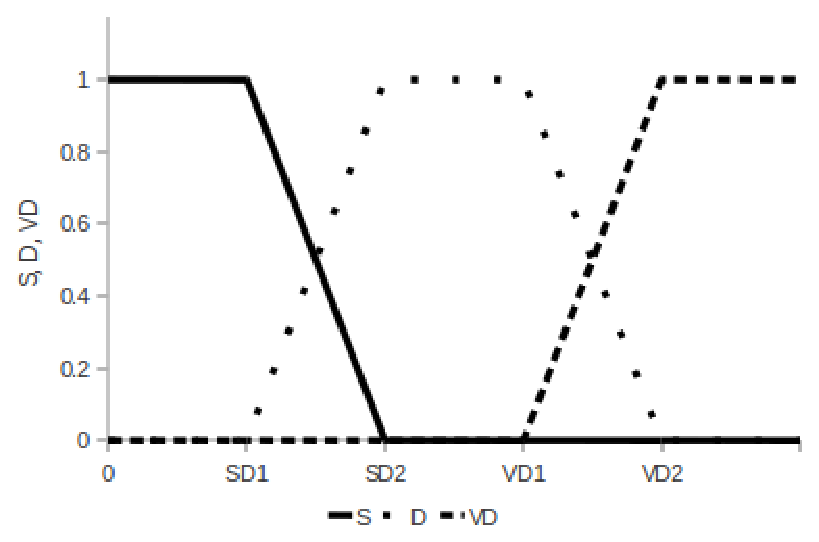
\includegraphics[width=0.5\textwidth]{similarity}
  \caption[The fuzzy variable Similarity]{The fuzzy sets $S$, $D$ and $VD$ corresponding respectively to the linguistic concepts $Similar$, $Different$ and $Very Different$ are called the $states$ of the fuzzy variable  $Similarity$. The limits $SD1$, $SD2$, $VD1$, $VD2$ are application specific.}
  \label{fig:similarity}
\end{figure}

The parameter $\alpha$ is the average distance  between agents and this changes at each step further influencing the fitness function. The parameter $\lambda$ influences the agents' activation pressure and it may decrease over time. The parameter $t$ is used for the  termination condition which could be something like \begin{math} t < t_{max}  \end{math}. The parameters $s_x, s_y$, the agent's vision limits may also be updated in some situations.  

\subsection{Experiments}
\label{sec:experiments}

In order to test the algorithm in a real-world scenario, the Iris dataset \cite{website:iris} was considered for a first test case. The data set contains 3 classes of 50 instances each, each class referring to a type of iris plant. There are 4 attributes plus the class: sepal length in cm, sepal width in cm, petal length in cm, petal width in cm, class (Iris Setosa, Iris Versicolour, Iris Virginica). This dataset is appropriate for rather testing classification, but it was preferred for clustering too because the class attribute is given and hence there is a way to evaluate the algorithm. So apparently it would be ideal for the algorithm to produce 3 clusters of 50 instances, the 3 clusters corresponding to the given 3 classes. 

The last 2 attributes (petal length in cm and petal width in cm) are highly correlated according to \cite{website:iris}. However we do not dismiss any of these attributes because we would like to keep as much of the data unchanged. We do however scale the data to the interval $[0, 1]$. At this point the clustering process can be started. In the final grid configuration one would clearly see the clustered agents. Due to space limitations we can't show here the final grid configuration, but we will immediately summarize the results.
Besides the final grid configuration a membership table is also produced. The membership table shows the membership degree of each agent to the clusters. Relevant parts of the membership table will also be explained immediately. 

According to the Iris dataset \cite{website:iris}, items ranging from $0$ to $49$ belong to the first class, items ranging from $50$ to $99$ belong to the second class and items ranging from $100$ to $149$ belong to the third class. So from the grid table it appears that the following clusters contain some misclassifications:
\begin{itemize}
\item $Cluster1$ (items $0$ -- $49$): no misclassifications
\item $Cluster2$ (items $50$ -- $99$): 106, 119, 133, 134
\item $Cluster3$ (items $100$ -- $149$): 70, 77 
\end{itemize}
So it appears that the algorithm has misclassified $6$ items. 

Let us check each item in more detail. In order to do this deeper analysis we have to check out the membership degrees table. In the membership table one can see in what degree does each item belong to the clusters. This membership is computed with respect to the cluster representatives. The representative of a cluster is either the first item from that cluster or an item designated by the data analyst. In case of cluster merging if any of the representatives is designated by data analyst then this will be the representative of the new cluster; otherwise the representative of the cluster with the greatest number of elements will be chosen as the new representative. 
The agents $45$, $95$, $145$ resulted from this process as final representatives for clusters $1$, $2$ and $3$ respectively.

In the following, the similarity between each of the above reported misclassification and the corresponding representative is given. The membership degree to each cluster is also considered. The Euclidean distance between items has been used as a similarity metric. So a small similarity value i.e. distance between two items means that the two items are similar, should stay together.
\begin{table}[h!]
\begin{tabular}{lllll}
\cline{1-5}
MisclassificationId & Similarity  & C1 & C2 & C3\\ 
\hline
106 & 0.25 & 0 & 0.95 & 0.84\\
119 & 0.24 & 0 & 0.96 & 0.83\\
133 & 0.19 & 0 & 1    & 0.89\\
134 & 0.24 & 0 & 0.96 & 0.82\\
\hline \\
\end{tabular} 
\caption{Cluster2 --- RepresentativeId (95)}
\label{tab:cluster2id95}
\end{table}

From the table~\ref{tab:cluster2id95} it can be seen  that the similarities between the considered items and the representative lie between $0.19$ and $0.25$. This makes them $S$ ($Similar$) with this item. The membership degree with $Cluster2$ suggests that these items belong to this cluster. However the membership degree with $Cluster3$ is also high. The highest membership degree is with $Cluster2$ though and because of this it could be claimed that the items are actually correctly classified with respect to the considered metric. However we believe that these items cannot be considered to strictly belong either to $Cluster2$ or to $Cluster3$ as they are clearly at the border of the two clusters so they belong to both. In this case we also believe that they should not be regarded as misclassifications.

Let us check the reported misclassifications from the third cluster.

\begin{table}[h!]
\begin{tabular}{lllll}
\cline{1-5}
MisclassificationId & Similarity   & C1 & C2 & C3\\ 
\hline
70 & 0.22 & 0.0 &    0.94 &   0.98\\
77 & 0.24  & 0.0 &   0.95 &  0.96\\
\hline\\
\end{tabular} 
\caption{Cluster3 --- RepresentativeId (145)}
\label{tab:cluster3id145}
\end{table}

Like the items from table~\ref{tab:cluster2id95}, the items from the table~\ref{tab:cluster3id145} should also not count as misclassifications for the same reasons from above. So, arguably, the algorithm has a $100\%$ classification accuracy for the considered dataset.

It may be observed that starting with item $50$ a lot of instances have high membership degrees to both $Cluster2$ and $Cluster3$. This suggests that the  members of these two classes are not linearly separable as mentioned in \cite{website:iris} so a clustering process could also merge these two clusters and hence report only two clusters instead of three. 

For the second case study the wine dataset \cite{website:wine} was considered. This dataset contains the results of a chemical analysis of wines grown in the same region in Italy but derived from three different wine growers. The analysis determined the quantities of 13 constituents found in each of the three types of wines. In \cite{website:wine} it is mentioned that the initial dataset had 30 attributes. So the current dataset has 13 attributes plus the class. There are $178$ instances grouped in three classes corresponding to the three wine growers. Items ranging from $1$ to $59$ belong to the first class, items from $60$ to $130$ belong to the second class and items from $131$ to $178$ belong to the third class. 

The same procedure as the one form the first case study was applied and the following misclassifications resulted from the final grid configuration:
\begin{itemize}
\item $Cluster1$ (items $0$ -- $58$): 63, 65, 66, 73, 78, 95, 98
\item $Cluster2$ (items $59$ -- $129$): 130, 134 
\item $Cluster3$ (items $130$ -- $177$): 83
\end{itemize}
From the above it appears that the algorithm has misclassified $10$ items. Moreover, the following items have not been classified, i.e., they remained in the collection $U$ of unclustered agents: $59$, $110$, $121$, $123$, $124$. So it appears that there are $15$ classification errors. But let us check out everything in more detail.

The agents $17$, $89$, $166$ are the final representatives for clusters $1$, $2$ and $3$ respectively.

In the following, the similarity between each of the above reported misclassification and the corresponding representative is given. The membership degree to each cluster is also considered. The Euclidean distance between items has been used as a similarity metric. So a small similarity value i.e. distance between two items means that the two items are similar, should stay together.

\begin{table}[h!]
\begin{tabular}{lllll}
\cline{1-5}
MisclassificationId & Similarity  & C1 & C2 & C3\\ 
\hline
63 & 0.63 & 0.87 & 0.83 & 0\\
65 & 0.42 & 1 & 0.99 & 0\\
66 & 0.64 & 0.86 & 0.83 & 0\\
73 & 0.61 & 0.89 & 0 & 0\\
78 & 0.69 & 0.81 & 0 & 0\\
95 & 0.69 & 0.81 & 0 & 0\\
98 & 0.51 & 0.99 & 0.8 & 0\\
\hline \\
\end{tabular} 
\caption{Cluster1 --- RepresentativeId (17)}
\label{tab:cluster1id17}
\end{table}

From the table~\ref{tab:cluster1id17} it can be seen  that the similarities between the considered items and the representative are bellow $0.7$. This makes them still $S$ ($Similar$) with this item. The membership degree with $Cluster1$ suggests that these items belong to this cluster. However the membership degree with $Cluster2$ is also high. The highest membership degree is with $Cluster1$ though and because of this it could be claimed that the items are actually correctly classified with respect to the considered metric. 

Let us check the reported misclassifications from the second cluster.

\begin{table}[h!]
\begin{tabular}{lllll}
\hline
\multicolumn{2}{c}{Cluster2 --- RepresentativeId (89)} \\
\cline{1-5}
MisclassificationId & Similarity  & C1 & C2 & C3\\ 
\hline
130 & 0.76 & 0 & 0 & 0\\
134 & 0.68 & 0 & 0.82 & 0.8\\
\hline \\
\end{tabular} 
\caption{Cluster2 --- RepresentativeId (89)}
\label{tab:cluster2id89}
\end{table}

In table~\ref{tab:cluster2id89}, it can be seen that item $134$ has a high membership degree to both $Cluster2$ and $Cluster3$. Again, the highest membership is with $Cluster2$, the cluster in which it was classified. So it could be considered that it is correctly classified with respect to the considered metric. According to the same criterion, item $130$ should not belong to any of the clusters, it should be labelled as an outlier. However it is incorrectly classified to $Cluster2$. 

Let us check the reported misclassifications from the third cluster.

\begin{table}[h!]
\begin{tabular}{lllll}
\cline{1-5}
MisclassificationId & Similarity  & C1 & C2 & C3\\ 
\hline
83 & 0.6 & 0 & 0.81 & 0.9\\
\hline \\
\end{tabular} 
\caption{Cluster3 --- RepresentativeId (166)}
\label{tab:cluster3id166}
\end{table}

In table~\ref{tab:cluster3id166}, it can be seen that item $83$ has a high membership degree to both $Cluster2$ and $Cluster3$, but the highest membership is with $Cluster3$, the cluster in which it was classified. Again it could be considered that it is correctly classified with respect to the considered metric. So up to this point only the item $130$ was incorrectly classified to $Cluster2$.

Let us now analyse the items from the collection $U$ of unclustered items.

\begin{table}[h!]
\begin{tabular}{lllllll}
\cline{1-7}
ItemId & SimC1 & C1 & Sim C2 & C2 & Sim C3 & C3\\ 
\hline
59 & 1.06 & 0 & 0.75 & 0 & 1.08 & 0\\
110 & 0.91 & 0 & 0.93 & 0 & 1.11 & 0\\
121 & 0.73 & 0 & 0.96 & 0 & 1.2 & 0\\
123 & 1 & 0 & 0.9 & 0 & 0.99 & 0\\
124 & 0.94 & 0 & 0.86 & 0 & 1.13 & 0\\
\hline \\
\end{tabular} 
\caption{Unclustered items}
\label{tab:unclustered}
\end{table}

As it can be seen from the Unclustered items table, all the elements from the collection $U$ have very high similarity values with respect to each cluster and this implies membership degrees equal to zero. So these items are correctly left apart of any cluster. 

Consequently, it can be argued that only item $130$ is truly a misclassification with respect to the considered metric. On the other hand, it is clear that the approach has $15$ classification errors if the results from \cite{website:wine} were to be taken ad litteram. This may suggest that another metric should be considered for computing the similarity between items. From a classification point of view, even in the most pessimistic result interpretation ($15$ classification errors), the accuracy would be $91\%$.


\section{Conclusions and future work}
\label{sec:clustconclusionsfw}

We have introduced in this chapter new agent-based unsupervised learning approaches based on our original papers \cite{Gaceanu10AnAdaptive,  Gaceanu11AContext, Gaceanu11AFuzzy, Gaceanu11ABio, Gaceanu11AnIncremental}. 

The algorithms presented in Section \ref{sec:asmbasedclustering} are based on the adaptive ASM approach from \cite{Chen04AnAdaptive}. The major improvement is that, instead to moving the agents at a randomly selected site, we are letting the agents choose the best location. Agents can directly communicate with each other --- similar to the approach from \cite{Chira07Stigmergic}. In \cite{Schockaert04Fuzzy}, the fuzzy IF-THEN rules are used for deciding if the agents are picking up or dropping an item. In our model we are using the fuzzy rules for deciding upon the direction and length of the movement. Moreover, in the approach from Section \ref{sec:contextaware} the agents are able to adapt their movements if changes in the environment would occur. Case studies for these approaches have been performed in Section \ref{sec:caseasm}. In order to test the algorithm in a real-world scenario, the Iris and Wine datasets have been considered \cite{website:iris, website:wine}. Experiments outline the ability of our approaches to discover hybrid data. 
In Section \ref{chap:incrementalclustering} an incremental clustering algorithm is introduced. Incremental clustering is used to process sequential, continuous data flows or data streams and in situations in which cluster shapes change in time. Such algorithms are well fitted in real-time systems, wireless sensor networks or data streams because in such systems it is very hard or even impossible to store the entire datasets in memory. The algorithm considers one instance at a time and it basically tries to assign it to one of the existing clusters. Only cluster representatives have to be maintained in memory so computation is both fast and memory friendly. 
We have seen in the tests from the incremental approach (Section \ref{sec:experiments}) that most of the apparently classification errors were actually items that have high membership degrees to more than one cluster. Nevertheless, in our opinion, it is again clear that we are dealing with hybrid data. Actually the hybrid nature of the data is suggested in \cite{website:iris} and in \cite{website:wine} and this is the main reason for choosing these datasets for our analysis. By using fuzzy methods such features of the data are easy to be observed. The fact that there are hybrid items could be an indication of the quality of data.

For each approach proposed in this chapter we have outlined the advantages and drawbacks and emphasised improvement possibilities and directions for further extension. 

As future research directions we intend to improve the approaches presented in this chapter, to extend the evaluation of the proposed techniques and to investigate the use of various metaheuristics in unsupervised learning.





